\section{和与差}
\label{sec:rvt-sums-differences}

两个随机变量相加或相减，平均与波动怎样变化，前面已经知道。$X,Y$可积时$\mathbb{E}[X\pm Y]=\mathbb{E}[X]\pm\mathbb{E}[Y]$，不需要独立；二阶矩有限时
\[
 \operatorname{Var}(X\pm Y)=\operatorname{Var}(X)+\operatorname{Var}(Y)\pm2\operatorname{Cov}(X,Y) .
\]
但这两个数不能确定$X\pm Y$的分布。第~\ref{sec:rvt-output-distribution}节的三张概率表中，$X+Y$的均值都是$1$，分布却完全不同。这一节求和与差的完整分布。

\subsection{和的分布}
\label{sec:rvt-sum-distribution}

\paragraph{沿斜线累计}
事件$X+Y=z$的原像是平面上的直线$x+y=z$。离散时把直线上各点的联合质量相加；有密度时，式~\eqref{eq:rvt-sum-completion}已经给出沿这条直线的积分。把积分变量记成$x$，两种情形写在一起，就是下面的定理。

\begin{theorem}[和的分布]
\label{thm:rvt-sum-distribution}
设$Z=X+Y$。若$(X,Y)$离散，联合质量为$p_{X,Y}$，则
\begin{equation}
 p_Z(z)=\sum_{x}p_{X,Y}(x,z-x) .
 \label{eq:rvt-discrete-sum}
\end{equation}
若$(X,Y)$有联合密度$f_{X,Y}$，则
\begin{equation}
 f_Z(z)=\int_{\mathbb{R}}f_{X,Y}(x,z-x)\,\mathrm{d}x .
 \label{eq:rvt-density-sum}
\end{equation}
若$X$与$Y$还相互独立，联合规律分解为边缘之积，上两式分别成为
\begin{equation}
 p_Z(z)=\sum_{x}p_X(x)\,p_Y(z-x),\qquad f_Z(z)=\int_{\mathbb{R}}f_X(x)\,f_Y(z-x)\,\mathrm{d}x .
 \label{eq:rvt-convolution}
\end{equation}
\end{theorem}

\begin{proof}
离散情形，事件$Z=z$按$X$的取值分解为互不相交的事件$\{X=x,\ Y=z-x\}$，相加即得式~\eqref{eq:rvt-discrete-sum}。密度情形，在式~\eqref{eq:rvt-sum-completion}中把$(X_1,X_2)$换成$(X,Y)$，并把补出的坐标取为$X$本身（逆映射$x=w$、$y=z-w$，Jacobian行列式的绝对值仍为$1$），再把积分变量$w$改记为$x$，即得式~\eqref{eq:rvt-density-sum}。独立时代入$p_{X,Y}=p_Xp_Y$或$f_{X,Y}=f_Xf_Y$。
\end{proof}

式~\eqref{eq:rvt-convolution}右端的两种运算分别称为\term{离散卷积}（discrete convolution）与\term{卷积}（convolution），记作$p_X*p_Y$与$f_X*f_Y$。式~\eqref{eq:rvt-density-sum}不需要独立，但需要联合密度；式~\eqref{eq:rvt-convolution}只用边缘，代价是独立的假设。第~\ref{sec:rvt-output-distribution}节的例子说明，没有独立时用边缘作卷积会得到错误的答案。

\paragraph{卷积的读法}
固定$z$，把$f_Y$左右翻转再右移$z$，得到函数$x\mapsto f_Y(z-x)$；它与$f_X$逐点相乘再积分，就是$f_Z(z)$。在两个均匀变量的例子里，两个函数都是高度为$1$的方块，乘积是两个方块重叠部分上的$1$，积分等于重叠的长度。$z$从$0$增加到$1$，重叠从$0$增加到$1$；$z$从$1$增加到$2$，重叠又减到$0$。这正是上一节算出的三角形密度。

图~\ref{fig:rvt-convolution-slide}画出$z=0.7$与$z=1.4$两个位置。按质量的语言，$f_Z(z)$收集了所有满足$x+y=z$的输入对的质量，每一对的权重是$f_X(x)f_Y(z-x)$；滑动的方块只是把“哪些$x$与$z-x$同时可能”画了出来。

\begin{BookInlineFigure}
  \centering
  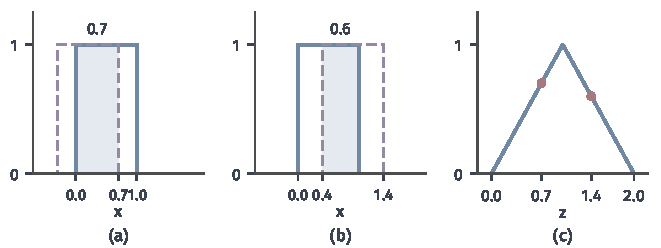
\includegraphics[width=112mm]{figures/07-probability/01-elementary-probability/matplotlib/rvt-convolution-slide/figure.pdf}
  \caption{卷积作为滑动重叠，$f_X=f_Y=\mathbf{1}_{(0,1)}$。(a)$z=0.7$：蓝色方块为$f_X$，紫色方块为翻转平移后的$f_Y(z-x)$，浅蓝重叠长度为$0.7$。(b)$z=1.4$，重叠长度为$0.6$。(c)$f_Z=f_X*f_Y$（蓝），红点是$z=0.7$与$z=1.4$处的值。}
  \label{fig:rvt-convolution-slide}
\end{BookInlineFigure}

\paragraph{骰子的卷积}
两枚骰子各自的质量是$\{1,\ldots,6\}$上的$1/6$。由式~\eqref{eq:rvt-convolution}，$p_Z(z)$等于$1/36$乘以满足$1\leq x\leq6$且$1\leq z-x\leq6$的整数$x$的个数。这些$x$从$\max(1,z-6)$到$\min(6,z-1)$，个数是$6-\lvert z-7\rvert$，与第~\ref{sec:rvt-output-distribution}节数格子的结果相同。

再与第三枚骰子作卷积，就得到三枚骰子之和的质量，取值从$3$到$18$。例如和为$10$时，把两枚之和的质量与第三枚的$1/6$相乘求和，得到
\[
 p_3(10)=\frac16\sum_{x=4}^{9}p_2(x)=\frac16\cdot\frac{3+4+5+6+5+4}{36}=\frac{27}{216}=\frac18 .
\]
卷积满足交换律与结合律，这对应于加法的次序不影响和；所以三枚骰子可以按任意次序逐个加入。图~\ref{fig:rvt-dice-convolution}显示，每多一次卷积，质量就向中间聚得更圆。

\begin{BookInlineFigure}
  \centering
  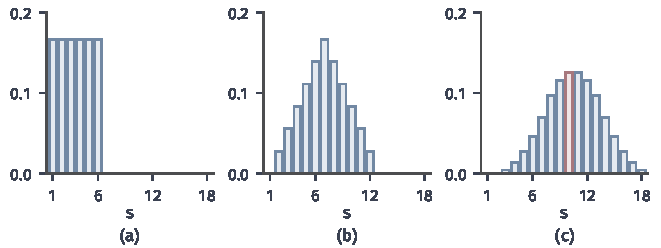
\includegraphics[width=112mm]{figures/07-probability/01-elementary-probability/matplotlib/rvt-dice-convolution/figure.pdf}
  \caption{骰子点数和的质量，由逐次离散卷积算出。(a)一枚；(b)两枚，三角形；(c)三枚，红色柱是和为$10$的质量$1/8$。}
  \label{fig:rvt-dice-convolution}
\end{BookInlineFigure}

连续的情形也一样。$n$个独立的$\operatorname{Unif}(0,1)$之和，$n=2$时是三角形，$n=3$时由三段二次多项式拼成，$n=4$时由四段三次多项式拼成，每加一次，曲线就光滑一阶。图~\ref{fig:rvt-uniform-sums}中，$n=4$时的密度已经和均值$2$、方差$4/12$的高斯密度非常接近。这种逼近在什么意义下、以什么速度成立，以及样本平均怎样集中到均值附近，是第~\ref{chap:laws-of-large-numbers}章与第~\ref{chap:central-limit-theorem}章的内容；这里只需要知道，每一步都是一次卷积。

\begin{BookInlineFigure}
  \centering
  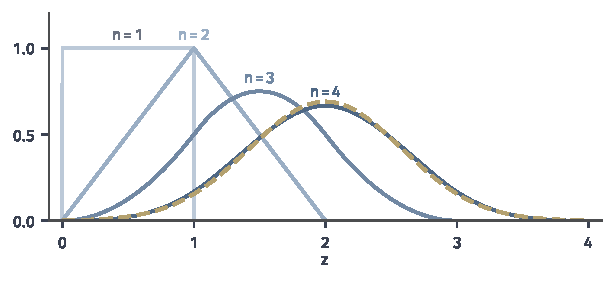
\includegraphics[width=104mm]{figures/07-probability/01-elementary-probability/matplotlib/rvt-uniform-sums/figure.pdf}
  \caption{$n$个独立$\operatorname{Unif}(0,1)$之和的密度，$n=1,2,3,4$（蓝色由浅到深），由逐次数值卷积算出。黄色虚线是均值$2$、方差$1/3$的高斯密度，与$n=4$的曲线对照。}
  \label{fig:rvt-uniform-sums}
\end{BookInlineFigure}

\paragraph{封闭的分布族}
有些分布族在独立相加下封闭：和仍在同一族中，参数按简单的规则相加。这能省去卷积计算，但每一条都有条件。

二项分布。设$X\sim\operatorname{Bin}(m,p)$与$Y\sim\operatorname{Bin}(n,p)$独立，成功概率相同，记$q=1-p$。由式~\eqref{eq:rvt-convolution}，$p$与$q$的幂次在每一项中都是$p^kq^{m+n-k}$，可以提出来：
\[
 p_Z(k)=\sum_{j}\binom{m}{j}p^{j}q^{m-j}\binom{n}{k-j}p^{k-j}q^{n-k+j}=p^{k}q^{m+n-k}\sum_{j}\binom{m}{j}\binom{n}{k-j} .
\]
最后的和数的是从$m+n$个对象中选$k$个、其中$j$个来自前$m$个的方法数，对$j$求和就是$\binom{m+n}{k}$。于是$X+Y\sim\operatorname{Bin}(m+n,p)$：$m$次试验接着$n$次试验，共$m+n$次。

成功概率不同时这条结论不成立。$\operatorname{Bin}(1,1/2)$与$\operatorname{Bin}(1,1/3)$独立相加，和的质量是
\[
 p_Z(0)=\frac13,\qquad p_Z(1)=\frac12,\qquad p_Z(2)=\frac16 .
\]
若它是$\operatorname{Bin}(2,r)$，由均值$2r=5/6$得$r=5/12$，于是应有$p_Z(0)=(7/12)^2=49/144$，与$1/3=48/144$不符。

Poisson分布。设$X\sim\operatorname{Poisson}(\lambda)$与$Y\sim\operatorname{Poisson}(\mu)$独立。卷积中提出$\mathrm{e}^{-(\lambda+\mu)}/k!$，剩下的和由二项式定理求出：
\[
 \begin{aligned}
 p_Z(k)&=\sum_{j=0}^{k}\frac{\mathrm{e}^{-\lambda}\lambda^{j}}{j!}\cdot\frac{\mathrm{e}^{-\mu}\mu^{k-j}}{(k-j)!}
 =\frac{\mathrm{e}^{-(\lambda+\mu)}}{k!}\sum_{j=0}^{k}\binom{k}{j}\lambda^{j}\mu^{k-j}\\
 &=\frac{\mathrm{e}^{-(\lambda+\mu)}(\lambda+\mu)^{k}}{k!} .
 \end{aligned}
\]
即$X+Y\sim\operatorname{Poisson}(\lambda+\mu)$，强度相加，参数不必相同。

高斯分布。设$X\sim\mathcal{N}(\mu_1,\sigma_1^2)$与$Y\sim\mathcal{N}(\mu_2,\sigma_2^2)$独立，$\sigma_1,\sigma_2>0$。由线性变换的结论，可以写成
\[
 X=\mu_1+\sigma_1Z_1,\qquad Y=\mu_2+\sigma_2Z_2 ,
\]
其中$Z_1,Z_2$独立且都是标准高斯。令$s=\sqrt{\sigma_1^2+\sigma_2^2}$。取第一行为$(\sigma_1,\sigma_2)/s$的$2\times2$正交矩阵$\bm{Q}$，由上一节的结论，$\bm{Q}\bm{Z}$的协方差是$\bm{Q}\bm{Q}^{\top}=\bm{I}$，与$\bm{Z}$同分布，所以它的第一个分量$(\sigma_1Z_1+\sigma_2Z_2)/s$服从$\mathcal{N}(0,1)$。于是
\begin{equation}
 X+Y=\mu_1+\mu_2+s\cdot\frac{\sigma_1Z_1+\sigma_2Z_2}{s}\sim\mathcal{N}\bigl(\mu_1+\mu_2,\ \sigma_1^2+\sigma_2^2\bigr) .
 \label{eq:rvt-gaussian-sum}
\end{equation}
直接计算卷积并对指数配方，也得到同样的结果。

Gamma分布与$\chi^2$分布。式~\eqref{eq:rvt-gamma-dirichlet}的第一个因子已经说明，同速率的独立Gamma变量之和服从$\operatorname{Gamma}(\alpha_0,\beta)$。因为$\chi^2_\nu=\operatorname{Gamma}(\nu/2,1/2)$，独立的$\chi^2$变量相加时自由度相加。再结合式~\eqref{eq:rvt-chi2-one}，$Z_1,\ldots,Z_\nu$独立标准高斯时
\begin{equation}
 Z_1^2+\cdots+Z_\nu^2\sim\chi^2_\nu,\qquad \nu=1,2,\ldots
 \label{eq:rvt-chi2-sum}
\end{equation}
$\nu=2$时与极坐标一段算出的$\operatorname{Exp}(1/2)$一致。

\paragraph{独立不能省}
封闭性中的独立不能换成“边缘属于同一族”。取$X\sim\mathcal{N}(0,1)$，再取与$X$独立、以各$1/2$的概率取$\pm1$的随机符号$S$，令$Y=SX$。由于$X$与$-X$同分布，
\[
 \mathbb{P}(Y\leq y)=\tfrac12\mathbb{P}(X\leq y)+\tfrac12\mathbb{P}(-X\leq y)=\Phi(y),
\]
$Y$也服从$\mathcal{N}(0,1)$。由$S$与$X$独立，
\[
 \operatorname{Cov}(X,Y)=\mathbb{E}[SX^2]=\mathbb{E}[S]\,\mathbb{E}[X^2]=0 ,
\]
两者不相关。

可是$X+Y=(1+S)X$：$S=-1$时它等于$0$，$S=1$时它等于$2X$。于是$\mathbb{P}(X+Y=0)=1/2$，和在$0$处有原子，不是高斯分布，更不是式~\eqref{eq:rvt-gaussian-sum}预言的$\mathcal{N}(0,2)$。图~\ref{fig:rvt-closure-counter}画出两者的分布函数。这里$X$与$Y$不相关但不独立，$(X,Y)$也不是联合高斯；只有联合高斯时不相关才推出独立，那是第~\ref{chap:multivariate-distributions}章的结论。

\begin{BookInlineFigure}
  \centering
  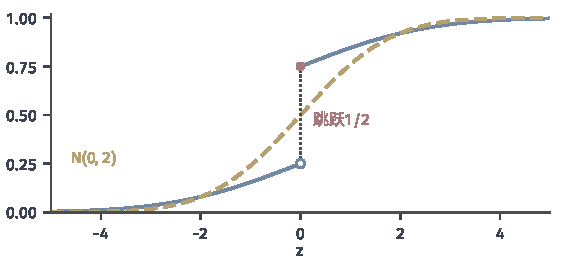
\includegraphics[width=96mm]{figures/07-probability/01-elementary-probability/matplotlib/rvt-closure-counter/figure.pdf}
  \caption{两个不相关的标准高斯之和。蓝线是$X+SX$的分布函数，它在$0$处跳跃$1/2$（红点），其余部分是$\tfrac12\Phi(z/2)$；黄色虚线是独立时的$\mathcal{N}(0,2)$分布函数。}
  \label{fig:rvt-closure-counter}
\end{BookInlineFigure}

\subsection{差的分布}
\label{sec:rvt-difference-distribution}

差可以看成和：$X-Y=X+(-Y)$。由线性变换的密度公式~\eqref{eq:rvt-linear-density}取$a=-1$，$-Y$的密度是$f_Y(-y)$，也就是把$f_Y$左右反射；离散时$-Y$的质量是$p_Y(-y)$。

\paragraph{反射后卷积}
把$-Y$代入定理~\ref{thm:rvt-sum-distribution}。一般情形下$X-Y=z$的原像是直线$y=x-z$，于是$f_{X-Y}(z)=\int f_{X,Y}(x,x-z)\,\mathrm{d}x$；$X$与$Y$独立时，$X$与$-Y$也独立（定理~\ref{thm:rvt-group-independence}），于是
\begin{equation}
 f_{X-Y}(z)=\int_{\mathbb{R}}f_X(x)\,f_Y(x-z)\,\mathrm{d}x .
 \label{eq:rvt-difference-density}
\end{equation}
离散时把积分换成求和。

两枚骰子之差$D=X_1-X_2$取$-5$到$5$的整数。与和的计算相同地数格子，或用离散版的式~\eqref{eq:rvt-difference-density}，得到
\[
 \mathbb{P}(D=d)=\frac{6-\lvert d\rvert}{36},\qquad d=-5,\ldots,5 .
\]
它与和的质量形状相同，只是中心从$7$移到$0$。两个独立$\operatorname{Unif}(0,1)$之差的密度同样是三角形，即$(-1,1)$上的$1-\lvert z\rvert$。

\paragraph{依赖改变差}
差对依赖关系很敏感。设$U,V$都服从$\operatorname{Unif}(0,1)$，比较三种联合规律：
\begin{itemize}
 \item $U,V$独立：$U-V$的密度是$1-\lvert z\rvert$，方差$1/6$；
 \item $V=U$：$U-V$恒为$0$，全部质量是一个原子，方差$0$；
 \item $V=1-U$：$U-V=2U-1\sim\operatorname{Unif}(-1,1)$，方差$1/3$。
\end{itemize}
三种情形的方差都符合
\[
 \operatorname{Var}(U-V)=\tfrac1{12}+\tfrac1{12}-2\operatorname{Cov}(U,V),
\]
协方差分别是$0$、$1/12$、$-1/12$。

协方差项前的负号有直接的解释。正相关时两个变量倾向于同时偏大或同时偏小，偏差在相减时相互抵消，差的波动变小；负相关时一个偏大另一个就偏小，相减反而叠加。和的情形正好相反，所以$\operatorname{Var}(X+Y)$中协方差项带正号。

联合高斯的情形可以写出完整的分布。设$(X,Y)$联合高斯，两个边缘都是$\mathcal{N}(0,1)$，相关系数为$\rho$。联合高斯向量的线性组合仍是高斯（第~\ref{chap:multivariate-distributions}章），由方差公式得到
\[
 X-Y\sim\mathcal{N}(0,\,2-2\rho),\qquad X+Y\sim\mathcal{N}(0,\,2+2\rho) .
\]
$\rho=0.8$时差的方差是$0.4$，$\rho=-0.8$时是$3.6$。图~\ref{fig:rvt-difference-dependence}把两组例子放在一起：边缘完全相同，只是联合规律不同，差的分布就从一个点变成三角形，再变成一段平坦的区间。

\begin{BookInlineFigure}
  \centering
  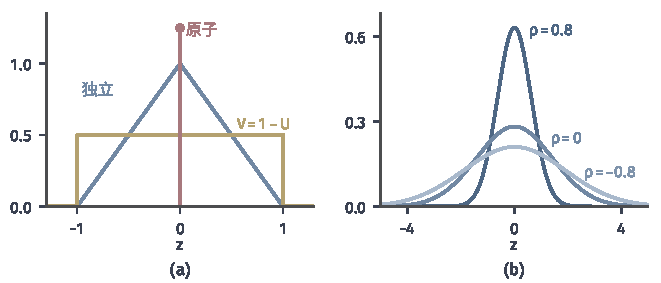
\includegraphics[width=112mm]{figures/07-probability/01-elementary-probability/matplotlib/rvt-difference-dependence/figure.pdf}
  \caption{相同边缘、不同依赖下的差。(a)$U,V\sim\operatorname{Unif}(0,1)$：独立时$U-V$的密度（蓝，三角形），$V=1-U$时的密度（黄，平坦），$V=U$时$0$处的原子（红色竖线，质量$1$）。(b)联合高斯、标准边缘、相关系数$\rho=0.8,0,-0.8$时$X-Y$的密度（蓝色由深到浅），方差分别为$0.4$、$2$、$3.6$。}
  \label{fig:rvt-difference-dependence}
\end{BookInlineFigure}

所以，和与差的分布由联合规律决定；均值与方差由边缘和协方差决定；只有在独立时，完整分布才能由边缘的卷积算出。
